\chapter{Editing atomic structures}\label{ch:modeling}

\chapterlead{A calculation-ready structure needs more than the right elements and atomic positions: it must also represent periodicity, connectivity, and the unit cell correctly. This chapter begins with a silicon cell, introduces selection, editing, and saving, and then combines the tools in worked examples involving a supercell, a vacancy, aromatic molecules, and ethanol.}

\section{Understand the structure model}

\subsection{Crystals and molecules}
\index{Molecular modeling}

A crystal model describes a periodic material through a unit cell and the atoms within it. Its three lattice vectors, $\mathbf a$, $\mathbf b$, and $\mathbf c$, define the cell's size and shape. They need not be perpendicular. In an oblique cell, moving along a lattice direction is different from moving horizontally or vertically on the screen.

A molecular model is usually a finite collection of atoms with explicit chemical bonds. For ethanol, for example, the model must specify which atoms are connected and whether each connection is a single or double bond. Two atoms that look close together on screen do not necessarily have the connectivity needed for molecular editing. Check atomic positions and chemical bonds as two aspects of the same model.

When a 3D structure document is active, the ribbon displays \ui{Crystal Modeling} or \ui{Molecule Modeling} according to the object type. Crystal tools cover cells, symmetry, defects, and surfaces; molecular tools cover sketching, chemistry, fragments, and geometry. Availability also depends on the selection. Setting a distance requires two atoms, and setting an angle requires three; a single selected atom is insufficient for either command.

To begin, open the \ui{Project Browser} from the sidebar, expand \ui{Structure}, and double-click the structure. Then select its modeling tab in the ribbon. If the project tree is hidden, choose \ui{Project Browser} from the sidebar's \ui{Open Panels} gallery. The sidebar controls working panels; the ribbon provides the structure commands used here.

\subsection{Cartesian and fractional coordinates}

Cartesian coordinates specify positions directly in space, usually in angstroms (\AA) in the modeling interface. Fractional coordinates give proportions along the three lattice vectors. For $(u,v,w)$, the position is $u\mathbf a+v\mathbf b+w\mathbf c$. These components are dimensionless: they specify how far to go along each lattice vector, rather than distances along global Cartesian axes.

To read the lattice input table, arrange the vectors as matrix rows:
\[
 A=\begin{bmatrix}
 a_x&a_y&a_z\\
 b_x&b_y&b_z\\
 c_x&c_y&c_z
 \end{bmatrix},\qquad
 \mathbf f=(u,v,w),\qquad \mathbf r=(x,y,z).
\]
The rows are $\mathbf a$, $\mathbf b$, and $\mathbf c$; the columns within each row are global $x,y,z$ components. With the row-vector convention used in this manual,
\begin{equation}
 \mathbf r=\mathbf f A,\qquad \mathbf f=\mathbf r A^{-1}.
 \label{eq:row-lattice-coordinates}
\end{equation}
Here $A^{-1}$ is the inverse of the complete lattice matrix, not the reciprocal of each entry. The cell must have nonzero volume for a Cartesian position to determine unique fractional coordinates.

For a simple example, take $\mathbf a=(4,0,0)$, $\mathbf b=(1,3,0)$, and $\mathbf c=(0,0,6)$, all in \AA. The fractional position $(0.5,0.5,0)$ gives
\[
 \mathbf r=0.5(4,0,0)+0.5(1,3,0)
          =(2.5,1.5,0)\,\text{\AA}.
\]
Half of $\mathbf b$ includes $0.5\,\text{\AA}$ along global $x$ and $1.5\,\text{\AA}$ along global $y$. The second fractional component of a skewed cell is therefore not its Cartesian $y$ coordinate. Figure~\ref{fig:round10-fractional-cartesian} shows the addition as two joined arrows.

\begin{figure}[!htb]
\centering
\begin{tikzpicture}[x=1mm,y=1mm,font=\sffamily\small]
 \fill[paleblue] (8,6)--(56,6)--(68,42)--(20,42)--cycle;
 \draw[teal,line width=.7pt] (8,6)--(56,6)--(68,42)--(20,42)--cycle;
 \draw[->,>=stealth,muted] (8,6)--(84,6) node[right] {$x$};
 \draw[->,>=stealth,muted] (8,6)--(8,49) node[above] {$y$};
 \draw[->,>=stealth,brand,line width=1pt] (8,6)--(32,6);
 \draw[->,>=stealth,brand,line width=1pt] (32,6)--(38,24);
 \draw[->,>=stealth,teal,line width=.8pt] (8,6)--(38,24);
 \draw[dashed,muted] (38,24)--(38,6);
 \fill[brand] (38,24) circle (1.2);
 \node[anchor=north,text=brand] at (22,5) {$u\mathbf a$};
 \node[anchor=west,text=brand] at (38,14) {$v\mathbf b$};
 \node[anchor=south east,text=teal] at (25,16) {$\mathbf r$};
 \node[anchor=north east] at (7,5) {$O$};
 \node[anchor=west,text=brand] at (42,27) {$\mathbf f=(u,v,0)$};
 \node[anchor=west,text=muted,font=\sffamily\footnotesize] at (78,35) {Cell cross-section};
 \node[anchor=west,text=muted,font=\sffamily\footnotesize] at (78,28) {Add vectors for position};
 \node[anchor=north,text=teal] at (54,4) {$\mathbf a$};
 \node[anchor=east,text=teal] at (15,31) {$\mathbf b$};
\end{tikzpicture}
\caption{Fractional and Cartesian coordinates (2D schematic). Adding $u\mathbf a$ and $v\mathbf b$ gives $\mathbf r$. In a skewed cell, $\mathbf b$ has both global $x$ and $y$ components.}
\label{fig:round10-fractional-cartesian}
\end{figure}


In a cubic cell of side $5\,\text{\AA}$, $(0.5,0,0)$ instead gives a displacement of $2.5\,\text{\AA}$ along $\mathbf a$. The lattice differs, not the conversion rule. Holding $\mathbf f$ fixed while changing $A$ generally moves atoms with the cell. To keep their spatial positions fixed, retain $\mathbf r$ and recalculate $\mathbf f$ using the new lattice. Section~\ref{sec:lattice-transform-reference} in Chapter~\ref{ch:modeling-tools} explains these options.

\begin{table}[!htb]
\centering\small
\begin{tabularx}{\linewidth}{llX}
\toprule
Symbol & Units & Meaning in the parameters\\
\midrule
$A$ & \AA & Lattice matrix with rows $\mathbf a,\mathbf b,\mathbf c$.\\
$\mathbf f$ & Dimensionless & Fractional coordinates along the lattice vectors.\\
$\mathbf r,\mathbf p$ & \AA & Cartesian position and a rotation anchor or point on a mirror plane.\\
$\mathbf n,\hat{\mathbf n}$ & Direction & A nonzero direction vector and its unit vector; direction alone is not a length in \AA.\\
$\theta$ & Degrees & Dialog rotation angle, positive by the right-hand rule.\\
$S$ & Integers & Supercell transformation matrix defining the new lattice.\\
$N,V$ & Count, \AA$^3$ & Independent model-site count and cell volume.\\
$\varepsilon_a,\varepsilon_b,\varepsilon_c$ & Dimensionless & Relative extension along the three lattice vectors.\\
\bottomrule
\end{tabularx}
\caption{Symbols used in modeling formulas. Coordinates and anchors have length units; direction vectors specify orientation. Their roles in dialogs differ.}
\label{tab:round10-modeling-symbols}
\end{table}


After selecting an atom, use the information card in the 3D view to check its position. A displayed periodic image may lie in a neighboring cell; its image offset identifies that translation. Before entering three numerical components, check the coordinate type. A displacement of $0.5\,\text{\AA}$ is not the same as half a lattice vector.

\Needspace{7\baselineskip}
\begin{notebox}{Atom indices}
Atom indices in modeling dialogs start at 1. They identify sites in the current document and are different from atomic numbers. Index 6 might identify the sixth silicon atom; it does not mean carbon. Check the indices again after changing the atom count or reordering the model.
\end{notebox}

\section{Example: inspect a silicon cell}

This example uses \mbox{\file{Si.poscar}} from the accompanying examples. It contains 8 silicon atoms in a cubic cell with a side length of approximately $5.46873\,\text{\AA}$. That lattice constant is the starting parameter for this modeling exercise.

The silicon calculation in Chapter~\ref{ch:workflows} uses a different file, \file{silicon.cif}, with a side length of approximately $5.44370\,\text{\AA}$. Both contain 8 silicon sites, but their lattice constants differ. Use \mbox{\file{Si.poscar}} when checking supercell scaling here, and start from the specified file when comparing energies in the calculation chapters.

Open \file{Si-introduction.ks} saved in Chapter~\ref{ch:workspace}, then import \file{Si.poscar}. The project tree will contain both the original \file{silicon} and the newly imported \file{Si}. Perform the following operations in the \file{Si} document. Save the modeling work under a new project name to retain the original exercise.

\begin{steps}
  \item Open \file{Si-introduction.ks}, import \file{Si.poscar}, and open the new \file{Si} structure's 3D document. Wait for the atoms, cell, and information area to appear.
  \item Drag with the left mouse button to rotate and use the wheel to zoom. Inspect the whole cell first, then zoom in until individual atoms are easy to distinguish.
  \item Click an atom and inspect its site index, element, and coordinates. Select another atom and observe how the information changes.
  \item Use the viewer toolbar's axis controls to view the structure along different lattice directions. In a nonorthogonal cell, a lattice axis and its corresponding reciprocal axis can point in different directions; this becomes particularly useful when inspecting inclined surfaces.
  \item Press Space to recenter and fit the view. Rotating the view changes only the viewing direction, not the atomic positions.
\end{steps}

Figure~\ref{fig:si-periodic-image-inspection} shows the information card for a periodic image of Site 7. Subtracting the \ui{Image} offset from the displayed fractional coordinates gives the coordinates of the site in the model:
\[
 (0.750,0.250,1.250)-(0,0,1)=(0.750,0.250,0.250).
\]
The offset is a translation by one cell along $\mathbf c$. The Cartesian coordinates locate the displayed image. A fractional coordinate outside the range 0 to 1 does not add an independent site to the model. The viewer summary reads 8 sites and 41 atoms; the latter includes displayed images.

\begin{figure}[!htb]
\centering
% Original: 3024×1758; full card (55,743,845,1305), 790×562; approximately 254 ppi at 79 mm.
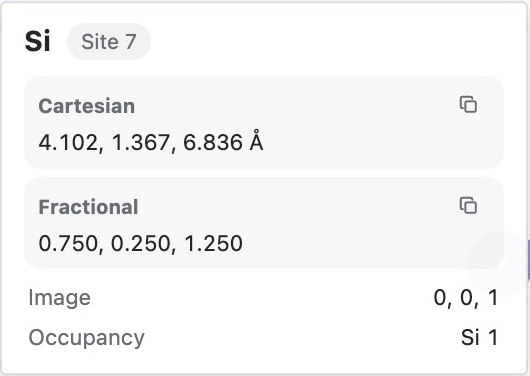
\includegraphics[width=79mm]{publication-assets/crop-4ce96785f91c44d963be.png}
\caption{Information card for a periodic image of Site 7. Read the fractional coordinates together with the image offset: this is still the model's seventh site. Si 1 under \ui{Occupancy} means full silicon occupancy.}
\label{fig:si-periodic-image-inspection}
\end{figure}

\subsection{Display more cells}

One cell may not show enough of the crystal's extended connectivity. Open the viewer settings from the 3D view's own toolbar, find \ui{Repeat cell}, and set the $a$, $b$, and $c$ repetitions to \mbox{2, 2, and 1}. More periodic images appear, making the spatial arrangement easier to inspect. Use the reset control afterward to return to $1\times1\times1$.

This setting changes only the displayed repetition range. It does not turn the eight-atom project structure into a larger calculation model. To model a local defect or reduce interactions between its periodic images, use \ui{Build Supercell}, described below. Both operations can put more atoms on screen, but they change different things.

\subsection{Choose a representation}

Ball-and-stick views make connectivity easy to see; larger spheres help show the space occupied by atoms. Viewer settings provide element colors, radius modes, atom scaling, and visibility controls for bonds, cell edges, coordination polyhedra, and other objects. When preparing a teaching figure or report, decide what the figure should explain before choosing a representation. Showing every auxiliary object at once can obscure the local feature of interest.

Crystal bonds are often inferred from neighboring atoms. Changing the bonding strategy can change the displayed bonds without moving any atoms. For a molecule with explicit topology, prefer connectivity from the source file. For a crystal, interpret displayed bonds in the context of the coordination environment.

\section{Edit atoms precisely}

\subsection{Make the right selection}

Click to select an atom. Hold Shift or Ctrl while clicking to add or remove atoms from the selection. Double-click to select a connected structure. For larger models, press B and drag a box, or press L and drag a lasso. Cmd/Ctrl+A selects all; Esc exits the current tool or clears the selection.

The selection is not necessarily every visible sphere within an outline. Periodic display may show several images of the same underlying site. Before editing, check the selection count and site indices, especially when displaying more than one cell. Save frequently used groups as selection sets and recall them through \ui{Selection Sets}.

\begin{notebox}{Why sites and atoms differ}
The viewer's \ui{sites} count is the number of independent model sites. Its \ui{atoms} count includes images used to display boundaries and periodic connections. Check supercell scaling, element counts, and defects against the site count. An eight-site silicon cell may show more than eight spheres; after building a $2\times2\times2$ supercell, check for 64 sites rather than expecting exactly 64 visible spheres.
\end{notebox}

\begin{figure}[htbp]
\centering
\begin{tikzpicture}[x=1mm,y=1mm,font=\sffamily\small]
  \node[text=brand] at (21,42) {Two model sites};
  \node[text=brand] at (85,42) {Sites and images};
  \fill[paleblue] (5,0) rectangle (37,32);
  \fill[paleblue] (69,0) rectangle (101,32);
  \draw[teal,line width=.75pt] (5,0) rectangle (37,32);
  \draw[teal,line width=.75pt] (69,0) rectangle (101,32);
  \fill[brand] (5,0) circle (2.3);
  \fill[teal] (21,16) circle (2.3);
  \node[text=white,font=\sffamily\scriptsize] at (5,0) {A};
  \node[text=white,font=\sffamily\scriptsize] at (21,16) {B};
  \fill[brand] (69,0) circle (2.3);
  \fill[teal] (85,16) circle (2.3);
  \node[text=white,font=\sffamily\scriptsize] at (69,0) {A};
  \node[text=white,font=\sffamily\scriptsize] at (85,16) {B};
  \foreach \x/\y in {101/0,69/32,101/32} {
    \draw[fill=white,draw=brand,line width=.8pt] (\x,\y) circle (2.3);
    \node[text=brand,font=\sffamily\scriptsize] at (\x,\y) {A};
  }
  \draw[->,>=stealth,teal,line width=.75pt] (43,16) -- (61,16);
  \node[text=brand,font=\sffamily\footnotesize] at (52,23) {Periodic view};
  \node[text=ink,font=\sffamily\footnotesize,align=center] at (21,-8) {Only A and B are stored};
  \node[text=ink,font=\sffamily\footnotesize,align=center] at (85,-8) {Hollow circles: images of A};
\end{tikzpicture}
\caption{Independent sites and boundary images (2D schematic). Site A can appear on several periodic boundaries. Drawing more spheres does not add independent model sites.}
\label{fig:periodic-sites}
\end{figure}


For geometry operations where order matters, clear the selection and select atoms individually. Two atoms define a distance; three define an angle with the second atom at its vertex; four define a dihedral in sequence. A different order can define a different geometric quantity.

\subsection{Drag interactively or enter numerical values}

After selecting atoms, press G and drag to translate them, or R and drag to rotate them. Press X, Y, or Z during a transform to constrain its direction. Dragging is useful for arranging an approximate geometry. For an exact displacement, angle, or bond length, finish with the relevant numerical command.

\ui{Translate Atoms} takes a displacement vector, whereas \ui{Move Atoms} takes new coordinates. To move an atom from $(1,0,0)$ to $(2,0,0)$, either translate it by $(1,0,0)$ or set its new coordinates to $(2,0,0)$. Crystal commands also offer the relevant fractional or Cartesian representation; check that choice before entering values.

\ui{Rotate Atoms} requires an axis, angle, and anchor. Angles are in degrees, and the anchor is a point through which the rotation axis passes. To rotate a fragment about its attachment site, place the anchor near that site rather than leaving it at a distant origin. The preview will then show the intended motion more clearly.

\section{Apply and save structural changes}

Most parameter dialogs that modify a structure offer \ui{Preview}, \ui{Apply}, and \ui{Cancel}. Preview shows the geometric effect of the parameters. Apply commits the change to the current document's editing state. Saving writes that state into the project. After changing parameters, preview again. Cancel closes the dialog and restores the original view.

\begin{steps}
  \item Open the modeling command and check the selection and parameter units.
  \item Enter the parameters and click \ui{Preview}. Rotate or zoom the view to inspect the changed region.
  \item If the result is suitable, click \ui{Apply}. Otherwise change the parameters and preview again, or click \ui{Cancel} to restore the original view.
  \item Check the atom count, cell, or geometric values after applying. Use Cmd/Ctrl+Z to undo and Shift+Cmd/Ctrl+Z to redo.
  \item Save the project after a meaningful stage of work and give the model a clear name.
\end{steps}

\ui{Reset} in \ui{History} restores the structure from when the document was opened or last saved. It differs from the camera recenter control. Saving establishes the latest saved model as the editing baseline and clears the current undo history. Keep two clearly named project structures for a lasting comparison rather than relying solely on undo.

Analysis commands do not necessarily create a structure preview, and their output varies. \ui{Diagnose Molecule} checks valence, close contacts, and bond lengths without changing the structure; the graphical interface reports \ui{Molecule diagnostics completed.} on completion. Interpret the result alongside composition, connectivity, and measured geometry. Section~\ref{sec:molecule-manual-check} gives a checking procedure; MATLAB\regmark{} toolbox users can also inspect diagnostic data with the accompanying script.

\section{Example: a silicon supercell with one vacancy}

\subsection{Build the supercell}
\index{Supercells}

A supercell repeats a base cell along selected directions and includes all replicated atoms in a new model. Diagonal repetition $(n_x,n_y,n_z)$ multiplies both atom count and volume by $n_xn_yn_z$. Here an eight-site silicon cell becomes a $2\times2\times2$ supercell containing 64 independent sites. The input and repeat factors determine that count, providing a direct check.

\begin{steps}
  \item Return to the \file{Si} document imported from \file{Si.poscar}. Restore display repetitions to $1\times1\times1$ so that displayed images are not confused with model atoms.
  \item On \ui{Crystal Modeling}, open \ui{Supercell \& Lattice} in the \ui{Crystal \& Cell} section and choose \ui{Build Supercell}.
  \item Check the default \literalinput{2 2 2} under \ui{Supercell scaling} and click \ui{Preview}. Inspect the enlarged cell boundaries in all three directions. A message below the controls confirms that the preview is displayed.
  \item Click \ui{Apply} if the preview is correct.
  \item Check for 64 silicon sites and lattice vectors twice their original lengths. The illustrated summary reads 64 sites and 166 atoms; use the first number to check replication. Save a separate project now if you want to retain a defect-free supercell before creating a vacancy.
\end{steps}

A general supercell is defined by an integer matrix $S$. Each row specifies one new lattice vector as a combination of the original three. For example, the first row $(2,1,0)$ means $\mathbf a'=2\mathbf a+\mathbf b$. With row-vector lattices,
\begin{equation}
 A'=SA,\qquad V'=|\det S|V,\qquad N'=|\det S|N.
 \label{eq:supercell-count-volume}
\end{equation}
The entries of $S$ must be integers and its determinant nonzero. The magnitude $|\det S|$ is both the volume ratio and the multiplier of independent sites. $N$ always counts model sites, not extra boundary-image spheres. For three repeat counts, $S=\operatorname{diag}(n_a,n_b,n_c)$ reduces Eq.~\eqref{eq:supercell-count-volume} to their product. The silicon example uses $S=2I$, so $|\det S|=8$ and 8 sites become 64.

For a nondiagonal algebraic check,
\[
 S=\begin{bmatrix}2&1&0\\0&1&0\\0&0&1\end{bmatrix},\qquad
 \begin{cases}
 \mathbf a'=2\mathbf a+\mathbf b,\\
 \mathbf b'=\mathbf b,\quad \mathbf c'=\mathbf c.
 \end{cases}
\]
The determinant is 2. An eight-site input should produce 16 sites and twice the volume. The new outline can be skewed, while the local periodic arrangement is copied from the original. This differs from strain: choosing a larger repeat unit does not double every interatomic bond length.

\ui{Supercell scaling} accepts either three repeat integers or a full $3\times3$ matrix. Write out the new basis vectors, check the determinant, preview the outline, and verify the applied site count to distinguish reorientation from replication. Input \literalinput{1 1 1} gives $I$ and does not enlarge the model. The tool still wraps equivalent positions into the unit cell, which can help collect representatives lying outside it.


\begin{figure}[!htb]
\centering
% Original: 3024×1758; full dialog (670,585,2355,1455), 1685×870; approximately 351 ppi at 122 mm.
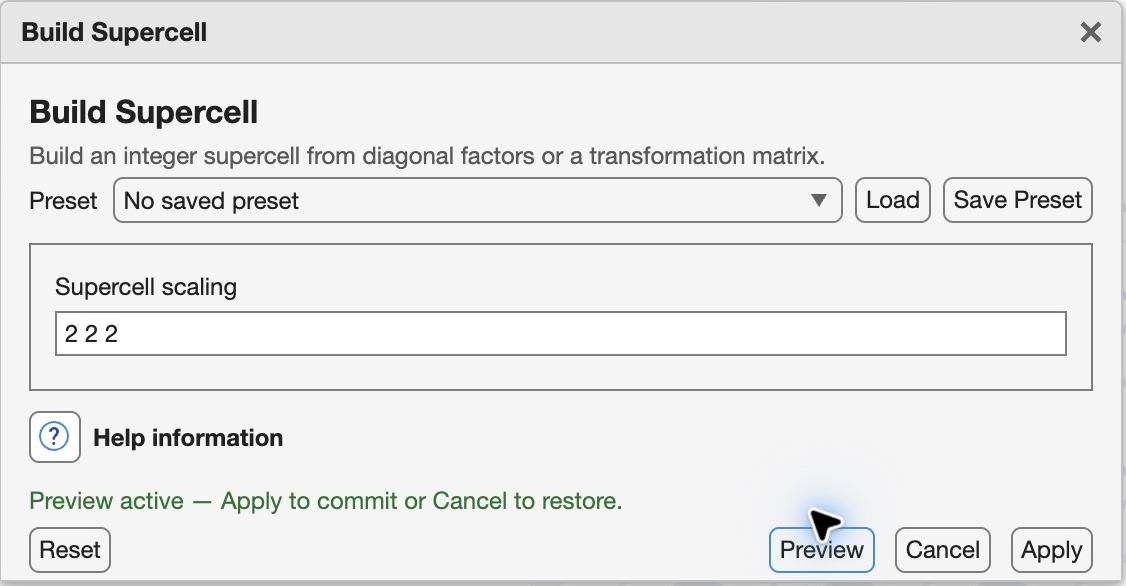
\includegraphics[width=\linewidth]{publication-assets/crop-0ff9d4164c5629316893.png}
\caption{Supercell parameters and preview status. \literalinput{2 2 2} repeats the cell twice in each direction.}
\label{fig:si-supercell-preview}
\end{figure}

\begin{figure}[!htb]
\centering
\begin{minipage}[b]{78mm}
% Original: 3024×1758; full model (875,365,2155,1615), 1280×1250; approximately 417 ppi at 78 mm.
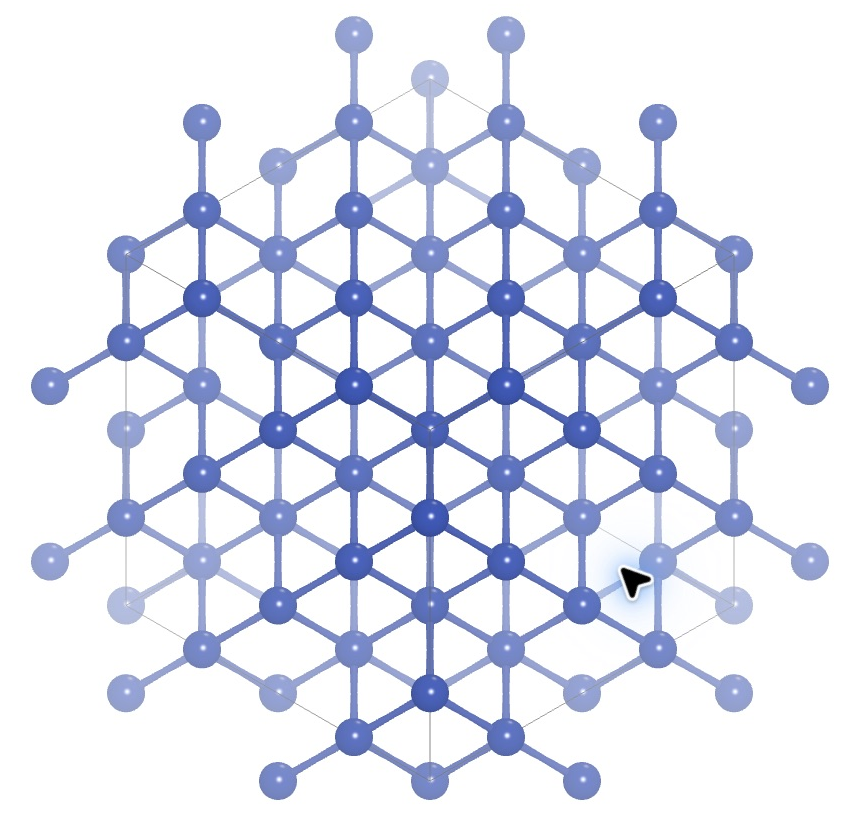
\includegraphics[width=\linewidth]{publication-assets/crop-0469f894473f746988e3.png}
\end{minipage}\hfill
\begin{minipage}[b]{42mm}
% Separate summary from the same image (45,330,465,560), 420×230; approximately 254 ppi at 42 mm.
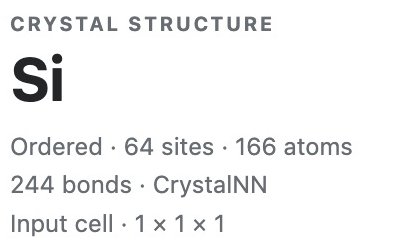
\includegraphics[width=\linewidth]{publication-assets/crop-c0154093dad09f77a9a2.png}
\end{minipage}
\caption{The applied silicon supercell, with the full model and a separate summary detail. The model contains 64 independent sites; the displayed count of 166 atoms includes boundary images. \ui{Input cell $1\times1\times1$} is the display range for the new supercell.}
\label{fig:si-supercell-result}
\end{figure}

\subsection{Create and check a vacancy}
\index{Vacancies}

A vacancy removes an atom from a lattice site. Expanding the cell first can reduce excessive interactions between neighboring periodic images of the defect. Determine the required supercell size through convergence tests for the subsequent calculation. Once the model is prepared, an appropriate calculation can be used to obtain the defect formation energy.

\begin{steps}
  \item Confirm that the active document is the 64-site \file{Si} supercell just created. This example removes site 1.
  \item On \ui{Crystal Modeling}, open \ui{Defects \& Alloys} in the \ui{Crystal Materials} section, then choose \ui{Create Point Defects → Vacancy}. In the dialog, check that \ui{Defect type} is \ui{Vacancy} and enter \file{1} under \ui{Site indices (MATLAB 1-based)}.
  \item Check the type and index, then click \ui{Apply}. Rotate the view to inspect the connections around the removed atom.
  \item Check that the site count falls from 64 to 63 while the supercell remains unchanged. The example reads 63 sites and 162 atoms; removing one independent site need not remove only one displayed image.
  \item Use \ui{Save As} to save \file{Si-vacancy-tutorial.ks}, retaining \file{Si-introduction.ks}. Check that the unsaved-change asterisk disappears from the title.
\end{steps}

\begin{figure}[!htb]
\centering
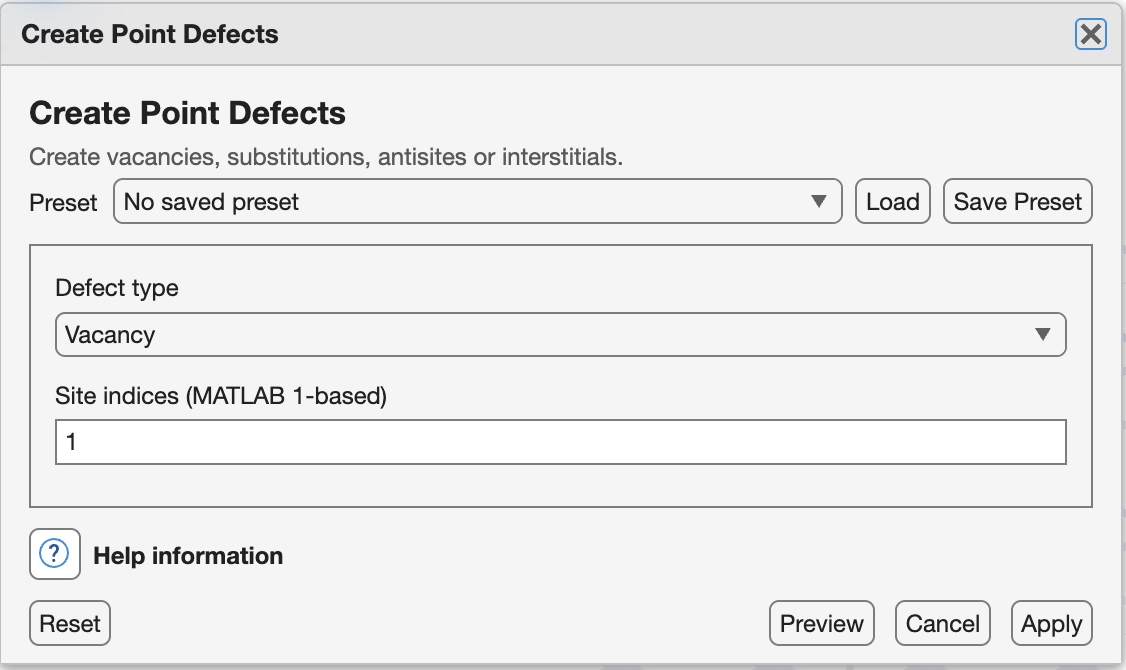
\includegraphics[width=113.7mm]{publication-assets/crop-601f9ce2a238baeb7b2e.png}
\caption{Silicon vacancy parameters: \ui{Vacancy} at site 1. After applying, check that the independent site count decreases from 64 to 63.}
\label{fig:si-vacancy-settings-result}
\end{figure}

The supplied \file{Si-vacancy-tutorial.ks} contains the original \file{silicon} reference and the vacancy-edited \file{Si} structure. For a defect-free comparison, rebuild the 64-site model from \file{Si.poscar} and save a separate project before creating the vacancy.

Symmetry handling in crystal editing affects equivalent positions. For a local defect, distinguish a change to one site from a change to an entire equivalent-site set. \ui{Create Point Defects} provides vacancy, substitutional, interstitial, and antisite operations. Check the independent site and element counts after applying.

\section{Example: build benzene and pyridine from an aromatic ring}
\index{Aromatic molecules}

\subsection{Build the benzene skeleton}

Molecular sketching can place atoms individually in the 3D view or build a skeleton quickly with rings and fragments. Press S to enter sketch mode. Click empty space to place an isolated atom, drag from an existing atom to add a connected atom, or drag to another existing atom to create a connection. The sketch toolbar selects elements, bond orders, and rings.

Here we first use the parameter dialog to create a regular six-membered ring, making the roles of aromaticity and hydrogen addition clear.

\begin{steps}
  \item Choose \ui{Home → Structure → New structure → Blank molecular structure}, activate the new document, and open \ui{Sketch Ring} on \ui{Molecule Modeling}.
  \item Set ring size to 6, element to C, and side length to $1.4\,\text{\AA}$. Enable the aromatic ring option. Enter 0, 0, 0 in the three center fields and 0, 0, 1 in the three normal fields.
  \item Leave attachment to other atoms disabled, then preview and apply. This creates the carbon skeleton; hydrogens still need to be added.
  \item Press Cmd/Ctrl+A to select the six ring atoms and run \ui{Add Hydrogens}. Check for the benzene composition $\mathrm{C_6H_6}$.
  \item Run \ui{Diagnose Molecule} and close its completion message. Rotate the view, inspect the ring, each carbon's hydrogen, and local distances, then save the model as \file{Benzene}.
\end{steps}

An aromatic ring has different connectivity information from a ring of ordinary single bonds. Arranging six carbons in a hexagon, or making their displayed bonds look alike, does not replace aromatic bonds and atomic chemistry settings. Check composition, bond order, and aromatic flags together.

Inspect the entire molecule from the side after adding hydrogens. A planar ring skeleton does not guarantee that automatically placed hydrogens lie in the ring plane. The supplied \file{benzene.json} preserves the initial hydrogenated model, while \mbox{\file{benzene-optimized.json}} contains the structure after generic molecular-model optimization. The latter is still a modeling reference. Use native JSON to exchange these aromatic molecules while preserving chemical properties and aromatic bonds, and check connectivity after reimporting.

\subsection{Replace one carbon with nitrogen}

Save the benzene model, then choose \ui{Home → Structure → Import structure from file...} and import \file{benzene.json} again. Use the new document for pyridine so that the original benzene remains available for comparison. To make hydrogen addition easy to check, remove hydrogens before replacing a ring carbon.

\begin{steps}
  \item Select all atoms in the newly imported structure and run \ui{Remove Hydrogens}. Select one ring carbon and open \ui{Atom Chemistry}.
  \item Change its element to N, set formal charge to 0 and hybridization to \file{sp2}, and retain the aromatic atom option.
\end{steps}

% Native English captures; see docs/provenance/english-edition-assets.json for source and crop metadata.
\begin{figure}[H]
\centering
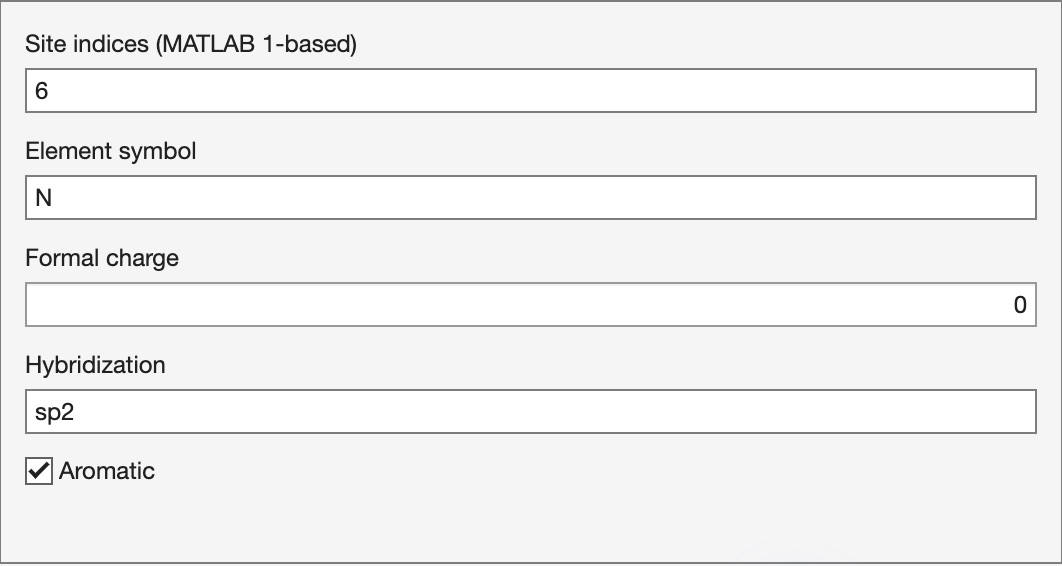
\includegraphics[width=\linewidth]{publication-assets/crop-f99354db0f163eccfd81.png}
\par\vspace{2mm}

\includegraphics[width=80mm]{publication-assets/crop-8ce96edd826deccee006.png}
\caption{Replacing ring atom 6 with nitrogen: element N, formal charge 0, hybridization \ui{sp2}, and \ui{Aromatic} enabled. The preview message appears below; click \ui{Apply} to commit.}
\label{fig:pyridine-chemistry}
\end{figure}


\begin{steps}[resume]
  \item Apply, select all ring atoms, and run \ui{Add Hydrogens}. Check for $\mathrm{C_5H_5N}$ and inspect connectivity around nitrogen.
  \item Run \ui{Diagnose Molecule}, close the completion message, and compare benzene and pyridine: composition, ring connectivity, and hydrogens near nitrogen. Import the supplied \file{pyridine.json} to compare with a complete neutral pyridine model.
\end{steps}

Element, formal charge, and hybridization hints together affect how connectivity is interpreted. Keeping every original hydrogen after changing an element can produce an unintended valence. Editing the skeleton first and adding hydrogens afterward is usually easier to check.

Neutral pyridine has 42 electrons; this example uses a singlet. Adding hydrogens to an odd-electron skeleton can retain the skeleton's spin multiplicity, causing a charge--spin mismatch when the file is read again. The supplied \file{pyridine.json} has charge 0 and multiplicity 1. Use it as a starting point for further calculations.

Figure~\ref{fig:pyridine-chemistry} shows the parameters used to change ring atom 6 to nitrogen. Figure~\ref{fig:pyridine-built-model} shows the completed six-membered ring and five hydrogens.

% Native English captures; see docs/provenance/english-edition-assets.json for source and crop metadata.
\begin{figure}[H]
\centering
% 不包含摘要；当前会话保留骨架多重度的现象由第7章正文另行说明。
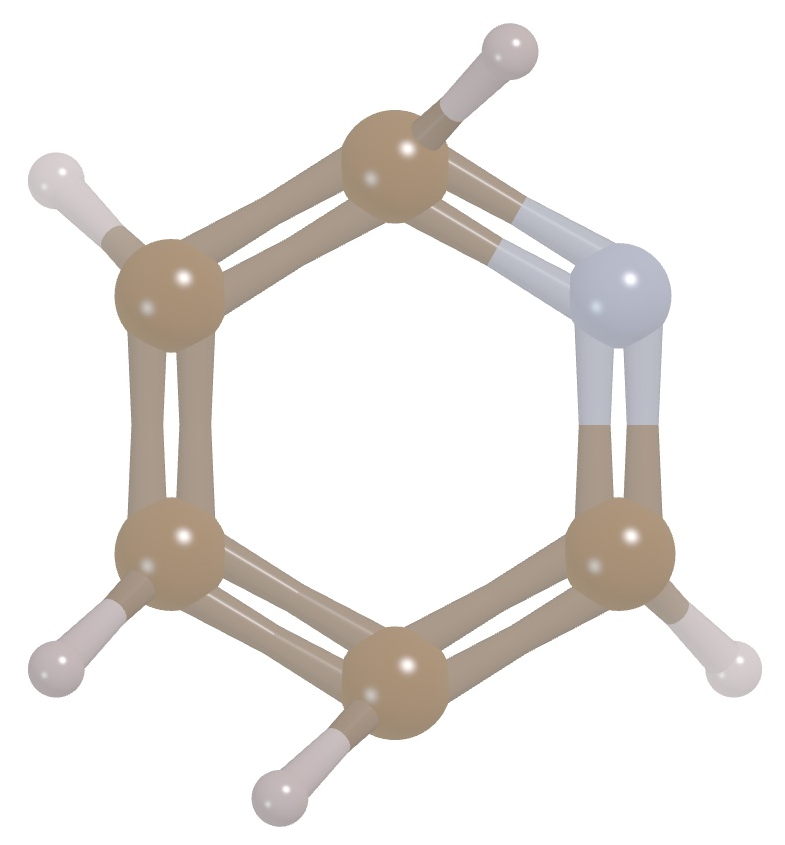
\includegraphics[width=70mm]{publication-assets/crop-60c8057a2bb7c31f0fd8.png}
\caption{Initial pyridine after element replacement and hydrogen addition to the six ring atoms: five carbons, one nitrogen, five hydrogens, 11 atoms in total, and 11 connections. For further calculations, use the neutral singlet structure in \file{pyridine.json}.}
\label{fig:pyridine-built-model}
\end{figure}


\section{Example: adjust an ethanol conformation}
\index{Molecular geometry}

\subsection{Build an initial molecule with clear connectivity}

Ethanol has a C--C--O heavy-atom skeleton. Choose \ui{Home → Structure → New structure → Blank molecular structure}, open the document, sketch the three atoms in sequence, and add hydrogens. The atom and bond commands provide an alternative. For readily checked input, this example uses the following coordinates in \AA.

\begin{table}[htbp]
\centering
\caption{Input for the ethanol skeleton. The collinear geometry is only a starting point for editing.}
\begin{tabularx}{\linewidth}{lX}
\toprule
Atom and index & Position and connection \\
\midrule
1: C & $(0,0,0)$; the first isolated atom.\\
2: C & $(1.52,0,0)$; connected to atom 1 by a single bond.\\
3: O & $(2.95,0,0)$; connected to atom 2 by a single bond.\\
\bottomrule
\end{tabularx}
\end{table}

With \ui{Use force-field ideal bond length} enabled, sketching uses an ideal bond length along the connection direction. Disable it to reproduce the table's coordinates exactly. Add hydrogens after building the skeleton and check for $\mathrm{C_2H_6O}$. This geometry has not yet been cleaned up; its collinear skeleton is not an equilibrium ethanol structure.

\subsection{Set geometric quantities}
\index{Distance measurements}
\index{Bond angles}
\index{Dihedral angles}

To read a distance, choose \ui{Measurements → Atom-to-atom distance} in the viewer toolbar and click atoms 1 and 2 in order. To change it, open \ui{Set Distance} in the ribbon, enter \literalinput{1 2} as the atom indices, and set the target to $1.52\,\text{\AA}$. Then open \ui{Set Angle}, enter \literalinput{1 2 3}, and set $109.5^\circ$. For the distance, angle, and dihedral operations here, choose the subtree movement scope so connected atoms move together.

The atoms scope moves local atoms only; subtree moves the connected atoms on one side; fragments adjusts a connected fragment as a whole. Changing an angle by moving a heavy atom without its attached hydrogens can distort neighboring geometry. Inspect the whole molecule in the preview rather than only the target angle.

\begin{steps}
  \item Set the required distances and angle in the C--C--O skeleton, measuring again after each application.
  \item Adjust the view and select four connected atoms in order, such as C--C--O--H. Check that the last atom is a hydrogen bonded to O.
  \item In \ui{Set Dihedral}, enter a convenient comparison angle, such as $60^\circ$, and preview the terminal fragment's rotation.
  \item Try another dihedral, inspect it, and undo to return to the earlier conformation. Use this comparison to understand conformational changes, rather than interpreting a chosen angle as the minimum-energy conformation.
\end{steps}

\subsection{Check an angle in the viewer}

Read edited geometric values in the 3D viewer's measurement card. \ui{Geometry Editor → Measure Geometry} in the ribbon is a separate command. Its graphical completion message reads \ui{Geometry measurement completed.} and does not list values in the dialog. Use the viewer procedure below to check an angle.

Figures~\ref{fig:ethanol-angle-parameters} and \ref{fig:ethanol-angle-measured} show angle setting and measurement. To make atom selection easier, this section imports a copy of \mbox{\file{ethanol-optimized.json}} and changes one angle. Its starting point differs from the earlier construction using a collinear skeleton.

\begin{steps}
  \item Import \mbox{\file{ethanol-optimized.json}} and open the copy's molecular document, retaining the original as a reference.
  \item In \ui{Set Angle}, enter atoms \literalinput{1 2 3}, target $109.5^\circ$, and movement scope \file{subtree}. Preview, then apply. This sets a geometric value directly; molecular optimization may follow later.
\end{steps}

% Native English captures; see docs/provenance/english-edition-assets.json for source and crop metadata.
\begin{figure}[H]
\centering
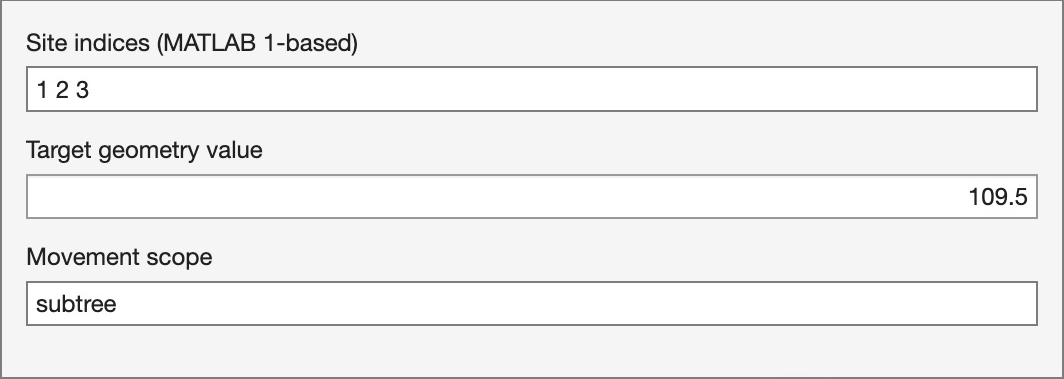
\includegraphics[width=\linewidth]{publication-assets/crop-0483f84ce4963946e315.png}
\par\vspace{2mm}

\includegraphics[width=80mm]{publication-assets/crop-17309e4ada4dd6ce532b.png}
\caption{Ethanol angle settings: atom sequence \literalinput{1 2 3}, target $109.5^\circ$, and movement scope \file{subtree}. The preview message appears below; click \ui{Apply} to commit the edit.}
\label{fig:ethanol-angle-parameters}
\end{figure}


\begin{steps}[resume]
  \item Close the parameter dialog. On the 3D view's right toolbar, open the ruler-shaped \ui{Measurements} button and choose \ui{Bond angle}. Select the atoms afresh after entering measurement mode.
  \item Click C atom 1, C atom 2, and O atom 3 in order; the second atom is the vertex. In the illustration, C1 is at the top, C2 is in the middle, and oxygen is red. After the third click, the left measurement card shows the angle and atom path, and two line segments and an arc appear on the model.
  \item Check for $109.500^\circ$ and the path \ui{\#1 C}, \ui{\#2 C}, \ui{\#3 O}. Record the value and atom order, close the card, and save the edited copy.
\end{steps}

This reading confirms that editing produced the specified angle. Ethanol's equilibrium angle must be determined by optimization. For a before-and-after comparison, measure the two separately saved models using the same atom order and record their actual readings.

% Native English captures; see docs/provenance/english-edition-assets.json for source and crop metadata.
\begin{figure}[H]
\centering
\begin{minipage}[t]{62mm}
\vspace{0pt}
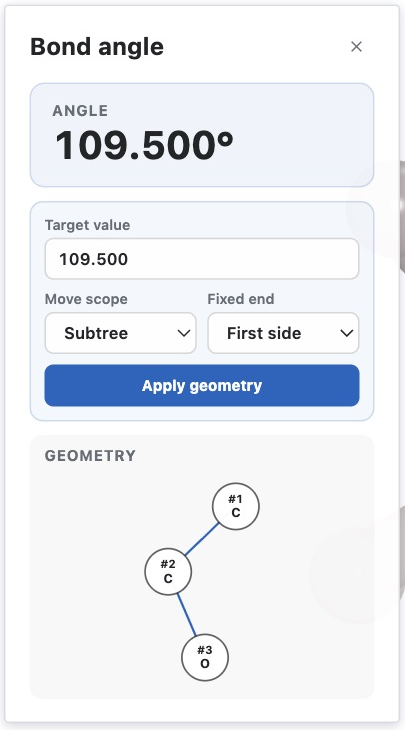
\includegraphics[width=\linewidth]{publication-assets/crop-cdb0f92bdcdbb307f144.png}
\end{minipage}\hfill
\begin{minipage}[t]{58mm}
\vspace{0pt}
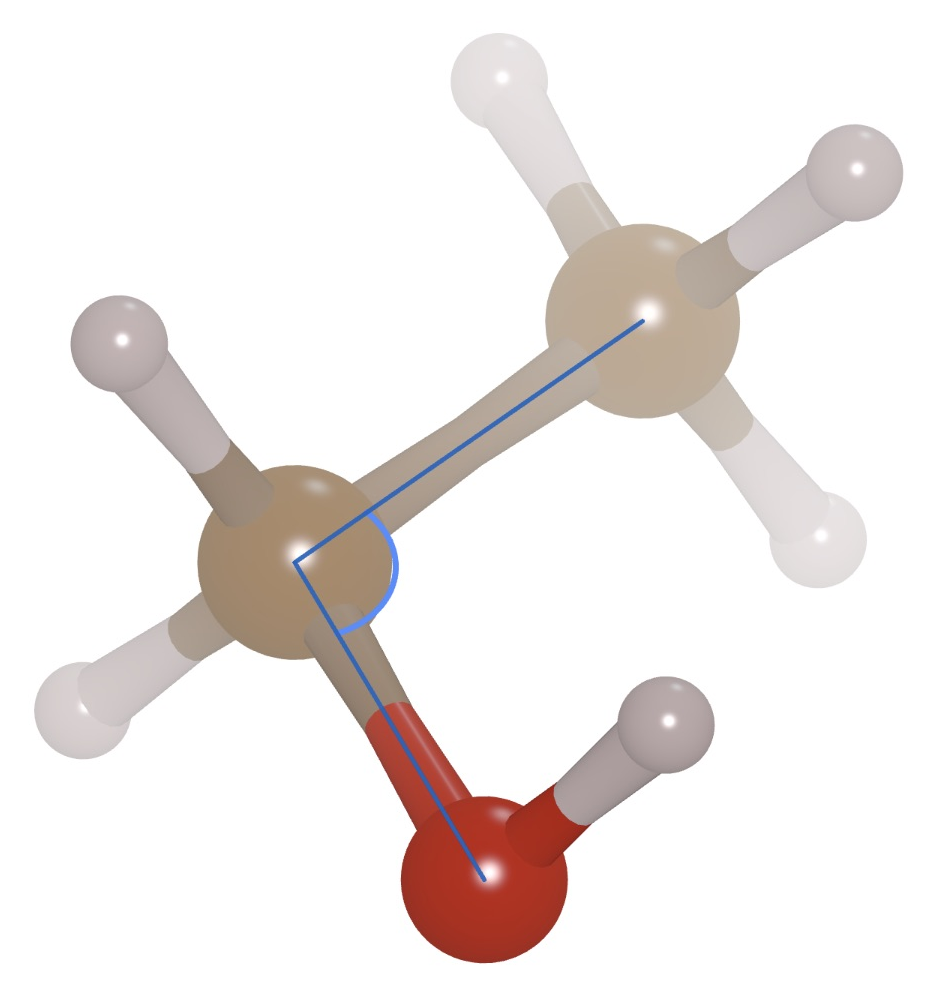
\includegraphics[width=\linewidth]{publication-assets/crop-4185f48c89b2b877f7b1.png}
\end{minipage}
\caption{Checking the edited angle with \ui{Bond angle}. Left: $109.500^\circ$ along \#1 C, \#2 C, and \#3 O. Right: the three heavy atoms and angle marker. The exercise starts from a copy of \file{ethanol-optimized.json} and sets the target to $109.5^\circ$; this is a prescribed exercise angle.}
\label{fig:ethanol-angle-measured}
\end{figure}


\subsection{Clean up and optimize the geometry}

\ui{Clean Geometry} applies rules to improve obvious local geometry problems. \ui{Optimize Geometry} further adjusts the structure using a generic molecular model. These tools are useful for initial preparation, especially after manual sketching or connectivity changes. Optimization parameters include an iteration limit, force tolerance, and optional fixed-atom indices.

Start with the defaults of 200 iterations and a 0.001 force tolerance. Preview and apply, compare the structural changes, and remeasure relevant bond lengths, angles, and close contacts. The accompanying script records the optimization method and convergence history in detail. For accurate equilibrium geometries, conformational energies, or reaction studies, continue with a suitable method from the calculation chapters.

The supplied \file{ethanol-edited.json} preserves the editing result. Reimporting gives a C--C distance of $1.52\,\text{\AA}$, a C--C--O angle of $109.5^\circ$, and a C--C--O--H dihedral of $60^\circ$ with atom 9 as the terminal hydrogen. \mbox{\file{ethanol-optimized.json}} has instead been cleaned and optimized with the generic molecular model, reaching a force threshold of $0.001\,\mathrm{kJ/(mol\,\text{\AA})}$ in 47 iterations. Optimization is free to change those geometric quantities; values set during editing are not automatically retained as constraints.

\subsection{Check molecular composition and geometry}\label{sec:molecule-manual-check}

Use the following sequence in the graphical interface, recording before-and-after readings together.

\begin{steps}
  \item Compare the formula and atom count in the structure summary with the intended molecule: $\mathrm{C_6H_6}$ for benzene, $\mathrm{C_5H_5N}$ for pyridine, and $\mathrm{C_2H_6O}$ for ethanol.
  \item Rotate the model and inspect each modified heavy atom and its attached hydrogens. Assess connectivity using the assigned elements, formal charges, bond orders, and aromaticity. To correct it, select the atom, explicitly adjust \ui{Atom Chemistry} or \ui{Set Bond Order}, then add hydrogens according to the connectivity.
  \item For a suspiciously short contact, choose \ui{Measurements → Atom-to-atom distance} and select two atoms in order. For an angle, choose \ui{Bond angle} and select three. Compare actual readings before and after editing rather than judging proximity from sphere sizes alone.
  \item Save the model and checking notes. Export native JSON for complete explicit bond and atom-property records. Run the accompanying checking script in the MATLAB\regmark{} toolbox environment when individual diagnostic data are needed.
\end{steps}

\ui{Diagnose Molecule} checks the entire molecule, regardless of a local selection. Compare edited models using composition, connectivity, and measurement records.

\section{Reuse modeling work}

Once a molecule is built, you need not start from individual atoms every time. Select an attachment site, open \ui{Fragment Sketcher} from its dropdown on \ui{Molecule Modeling}, choose the fragment and connection mode, and use \ui{Attach Fragment}. Check the fragment name and attachment head first. User fragments store reusable local structures in a library; repeat units serve polymer construction. They have different purposes.

Presets in parameter dialogs store frequently used settings, such as a supercell transformation or a combination of slab thickness and vacuum. Give them meaningful names, load them later, and adjust the values for the current material. Selection sets instead store groups of sites for repeated selection.

Use \ui{Record} and \ui{Save Recipe} for a longer sequence of operations. For research records and collaboration, keeping the original structure, operation parameters, and final files is easier to audit than retaining only a 3D screenshot. A figure explains the structure; a model file preserves its atoms and cell. Together they form a complete modeling result.
